% Sweave("flsp_man.rnw")
% pdflatex flsp_man.tex
% Manual for FLsp
% Front Guff
\documentclass[a4paper]{article}
\usepackage{geometry}
\usepackage{color}
\usepackage{framed}
\usepackage{setspace}
\usepackage{amsmath}
\usepackage{hyperref}
\usepackage{cite}
\usepackage{url}
\geometry{verbose,a4paper,tmargin=2cm,bmargin=1.5cm,lmargin=2cm,rmargin=3cm}
\definecolor{shadecolor}{rgb}{0.9,0.9,0.9}
\definecolor{darkblue}{rgb}{0,0,0.5}
\setlength{\parskip}{\medskipamount}
\setlength{\parindent}{0pt}
\onehalfspacing
\hypersetup{colorlinks, urlcolor=darkblue}

% Title page
\usepackage{Sweave}
\begin{document}

\title{FLsp - a Surplus Production model in FLR}
\author{ Finlay Scott <finlay.scott@cefas.co.uk\\
Cefas, Lowestoft, UK}
\date{June 2011}
\maketitle

% Intro. What it does
\section{Introduction}

This package implements the surplus production described in Polacheck REF.
At the moment only the model including observation error is implemented.
The Pella Tomlinson shape is used (which defaults to Schaeffer)
Tested against the three data sets in the paper.
Accurate gradients and hessian are returned using automatic differentiation (implemented using ADOLC REF)

% Details of the model being implemented
\section{The Model}
Following the Polacheck paper
Assumptions:
Observation error
Only r and k are estimated
sigma and q are approximated as described in the paper
The inital biomass is k

The general equation for the biomass through time is:
\begin{equation}
B_{y+1} = B_y + g(B_y) - C_y
%R = A_{y-1} / (\alpha + \beta A_{y-1})
\end{equation}

where $B$ is the stock biomass at the start of year $y$, $C$ is the catch during the year and $g$ is surplus production as a function of biomass.

Here we implement the Pella-Tomlinson form of surplus production:
\begin{equation}
g(B) = \frac{r}{p} B(1-(B/K)^p)
\end{equation}

where $r$ is the intrinsic growth rate parameter and $K$ is the average biomass level prior to exploitation.
By default, $p$ is set to 1 making the surplus prodution formulation the same as a Schaefer model.

The biomass is related to an index of abundance:
\begin{equation}
I_y = q B_y
\end{equation}

Where I is an index of relative abundance in year $y$ and $q$ is the catchability coefficient.

Here we assume that errors are introduced through observation. The population dynamics are assumed to be deterministic and all of the error occurs in the relationship between stock biomass and the index of abundance.
It is assumed that the error is multiplicative and log-normal with a constant coefficient of variation. The estimates of the model parameters are ($B_0$, $r$, $K$ and $q$) are obtained by maximising the likeilhood function:

\begin{equation}
L = \prod exp(\hat{v}_y^2 / (2\hat{\sigma}^2_v)) / (\sqrt{2\pi}\hat{\sigma}_v)
\end{equation}

where the product is over all years for which CPUE data are available and:

\begin{align}
\hat{v}_y &= log(C/E)_y - log(\hat{C/E})_y \\
\hat{\sigma}^2_v &= \sum\hat{v}_y^2 / n
\end{align}

where $n$ is the number of data points.

The value of $q$ which maximises the likelihood is given by:

\begin{equation}
\hat{q} = exp\left(\frac{1}{n} \sum_{y} log(I_y/\hat{B_y})\right)
\end{equation}

Following Polacheck et al $B_0$ is set to $K$. This means that only two parameters need to be estimated: $r$ and $K$.
In $FLsp$ the estimation is performed using the $DEoptim$ package REF.

\section{The FLsp class}

The $FLsp$ class extends the $FLModel$ class by including slots to store the catch and index time series. Catch is represented as an $FLQuant$ and index is represented as an $FLQuants$ object. This allows multiple indices to be used (not yet implemented).

To estimate the parameters $r$ and $K$, an $FLsp$ object must be created with catch and index data. The method $fitsp()$ is then called.
Once the object has been fitted, the biomass trajectory and other variables of interest (e.g. $sigma^2$ and $\hat{q}$ can be calculated).

\section{Creating and fitting FLsp objects}

Here we show how to create and fit a surplus production model using $FLsp$. The data set is New Zealand Rock Lobster, taken from Polcheck REF.

\begin{center}
\begin{minipage}[H]{0.95\textwidth}%
\begin{shaded}%
\begin{Schunk}
\begin{Sinput}
> # Load the library
> library(FLsp)
> # Load the New Zealand Rock Lobster data set
> data(nzrl)
> # This is a dataframe with year, catch and cpue
> # Take a look at the top of it
> head(nzrl)
> # Make FLQuant objects of the catch and cpue series
> catch <- FLQuant(nzrl$catch, dimnames=list(year=nzrl$year))
> index <- FLQuant(nzrl$cpue, dimnames=list(year=nzrl$year))
> # Create the FLsp object
> nzrl <- FLsp(catch=catch,index=index)
\end{Sinput}
\end{Schunk}
\end{shaded}%
\end{minipage}
\end{center}

After creating our object we are ready to fit the parameters.

\begin{center}
\begin{minipage}[H]{0.95\textwidth}%
\begin{shaded}%
\begin{Schunk}
\begin{Sinput}
> nzrl <- fitsp(nzrl)
\end{Sinput}
\end{Schunk}
\end{shaded}%
\end{minipage}
\end{center}

The published values for this data set are:
$r$ = 0.0659, 
$K$ = 129000, 
$\hat{q}$ = 2.461e-5, 
$\sigma$ = 0.207, 
$B_{current}$ = 21150. 
These can be compared to our results by interrogating the $FLsp$ object.
\begin{center}
\begin{minipage}[H]{0.95\textwidth}%
\begin{shaded}%
\begin{Schunk}
\begin{Sinput}
> # Look at the fitted parameters
> params(nzrl)
\end{Sinput}
\begin{Soutput}
An object of class "FLPar"
params
         r          k 
4.9429e-02 1.4233e+05 
units:  NA 
\end{Soutput}
\begin{Sinput}
> # qhat
> qhat(nzrl)
\end{Sinput}
\begin{Soutput}
An object of class "FLQuant"
, , unit = unique, season = all, area = unique

     year
quant 1         
  all 2.2129e-05

units:  NA 
\end{Soutput}
\begin{Sinput}
> # sigma2
> sqrt(sigma2(nzrl))
\end{Sinput}
\begin{Soutput}
An object of class "FLQuant"
, , unit = unique, season = all, area = unique

     year
quant 1      
  all 0.20695

units:  NA 
\end{Soutput}
\begin{Sinput}
> # returns the full biomass timeseries
> biomass(nzrl)
\end{Sinput}
\begin{Soutput}
An object of class "FLQuant"
, , unit = unique, season = all, area = unique

     year
quant 1945   1946   1947   1948   1949   1950   1951   1952   1953   1954  
  all 142335 141526 140712 139872 138632 136938 134522 132053 129201 125630
     year
quant 1955   1956   1957   1958   1959   1960   1961   1962   1963   1964  
  all 120818 116712 111203 107357 104214 101575  99251  96694  93644  90673
     year
quant 1965   1966   1967   1968   1969   1970   1971   1972   1973   1974  
  all  87703  84383  80786  77731  74500  71469  68528  65807  64061  62018
     year
quant 1975   1976   1977   1978   1979   1980   1981   1982   1983   1984  
  all  60105  58834  57229  55684  53941  51547  48982  46512  43729  40842
     year
quant 1985   1986   1987   1988   1989   1990  
  all  37370  33876  30495  27180  25139  22844

units:  NA 
\end{Soutput}
\end{Schunk}
\end{shaded}%
\end{minipage}
\end{center}

It can be seen that there is good agreement between the published results and those generated with $FLsp$. The differences are likely caused by the precision of the printed data set in the Polcheck paper (REF) and the fitting method used.

\section{Testing FLsp against the other data sets}

%There are two other data sets available: South Atlantic albacore ($saa$) and Northern Namibian hake ($nnh$). The above process can be repeated and the results checked against the published results (see Table~\ref{tab:compare3datasets}).

% HIDDEN!
%<<label=fitNAAandSAA,include=FALSE>>=

%TABLE OF RESULTS
\begin{table}
%% Tabular is not a floating environment so cannot caption it.
%% so put inside table, which is a floating environment
\begin{tabular}{|c|c|c|c|c|c|c|}
\hline
& \multicolumn{2}{|c|}{New Zealand Rock Lobster}
& \multicolumn{2}{|c|}{South Atlantic Albacore}
& \multicolumn{2}{|c|}{Northern Namibian Hake} \\
\hline
Measure & FLsp & Published & FLsp & Published & FLsp & Published \\
\hline
r          & 0.0494     & 0.0659    &  0.32     & 0.328 & 0.37     & 0.379     \\
K ('000 t) & 142     & 129.0     &  243     & 239.6  & 2820     & 2772.6    \\
$\sigma$   & 0.207 & 0.207     &  0.11 & 0.111  & 0.125 & 0.124     \\
$\hat{q}$  & 2.21e-05  & 2.461e-05 &  0.264  & 0.2671 & 0.000427  & 4.360e-04 \\
$B_{current}$  & 22.8  & 21.15 &  75  & 75.51 & 1660  & 1646.3 \\
MSY        &  0 & 2133.74 &  0  & 19.65 & 0  & 263.2 \\
\hline
\end{tabular}
\caption{Comparing the published results with those from $FLsp$ for three data sets.}
\label{tab:compare3datasets}
\end{table}

The results fitted with $FLsp$ are in good agreement with the published results.

\section{Plotting results}
There is no generic plot for FLsp at the moment. However, it is possible to look at the fitted index and residuals using relatively simple code. For example, to plot the indices with the fitted indices you can use (see Figure~\ref{fig:fitted_index_nzrl}):

\begin{center}
\begin{minipage}[H]{0.95\textwidth}%
\begin{shaded}%
%<<fig=FALSE,eval=FALSE, quiet=TRUE,echo=TRUE,results=verbatim,keep.source=TRUE>>=
% Why doesn't this line work here? Works further down
%<<label=nzrlfitedindexplotcode,include=FALSE>>= 
\begin{Schunk}
\begin{Sinput}
> fitted <- cbind(as.data.frame(nzrl@fitted_index),type="fitted")
> index <- cbind(as.data.frame(nzrl@index),type="index")
> index <- rbind(index,fitted)
> print(xyplot(data ~ year | qname, group=type, data=index, type="b",auto.key=TRUE))
\end{Sinput}
\end{Schunk}
\end{shaded}%
\end{minipage}
\end{center}

% Actually plot it
\begin{figure}
\begin{center}
%<<fig=TRUE,eval=TRUE, quiet=TRUE,echo=FALSE,results=hide,keep.source=FALSE>>=
%<<echo=FALSE, fig=TRUE, results=hide>>=
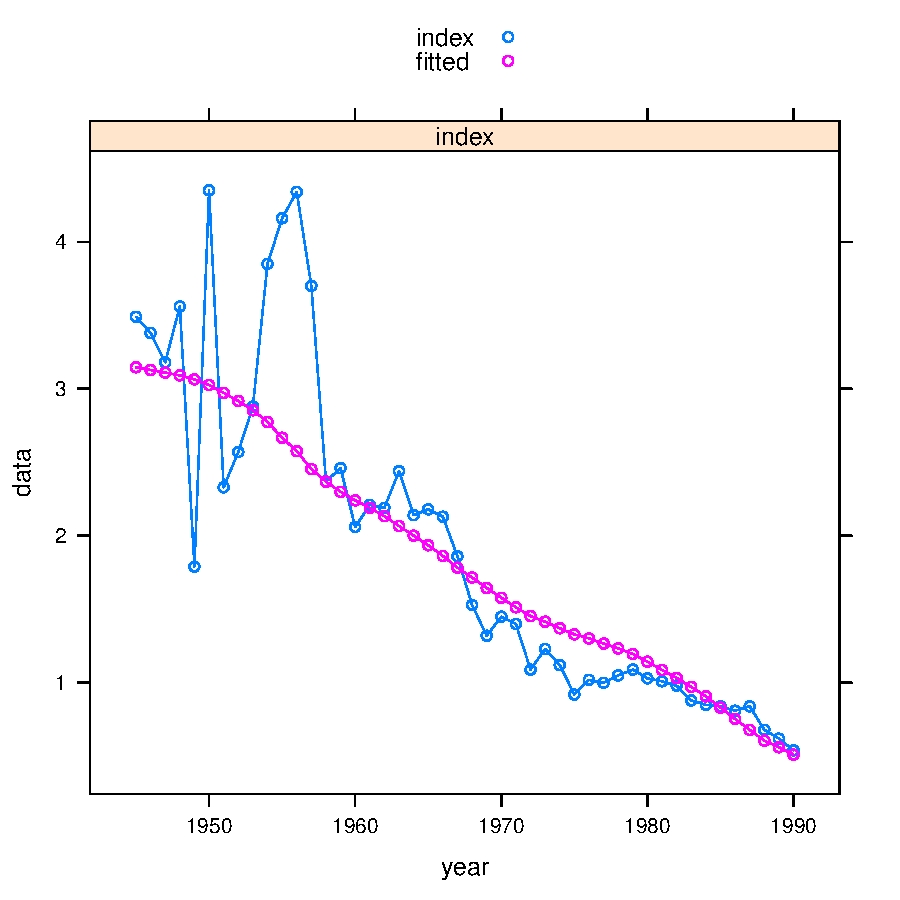
\includegraphics{flsp_man-nzrlfittedindexplot}
\end{center}
\caption{Indices and fitted indices for New Zealand rock lobster}
\label{fig:fitted_index_nzrl}
\end{figure}

To look at the residuals and put a loess function through them use (see Figure~\ref{fig:residuals_nzrl}):
\begin{center}
\begin{minipage}[H]{0.95\textwidth}%
\begin{shaded}%
%<<echo=TRUE, fig=FALSE, keep.source=TRUE,results=hide,eval=FALSE>>=
\begin{Schunk}
\begin{Sinput}
> residuals <- as.data.frame(nzrl@residuals_index)
> print(xyplot(data ~ year | qname, data = residuals, panel = function(x, 
+     y) {
+     panel.xyplot(x, y)
+     panel.loess(x, y, span = 1)
+ }))
\end{Sinput}
\end{Schunk}
\end{shaded}%
\end{minipage}
\end{center}

% Actually plot it
\begin{figure}
\begin{center}
%<<echo=FALSE, fig=TRUE, echo=FALSE>>=
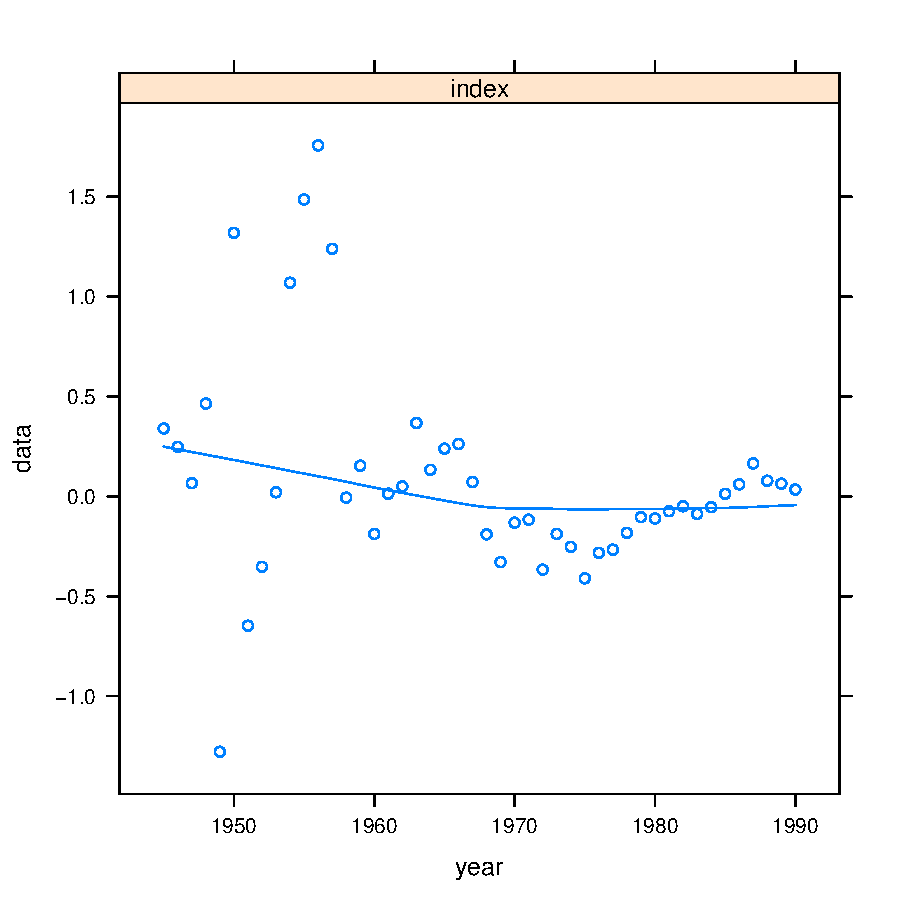
\includegraphics{flsp_man-nzrlresidplot}
\end{center}
\caption{Residuals for New Zealand rock lobster}
\label{fig:residuals_nzrl}
\end{figure}

\section{Profiling the fit}

You can explore how good the fit is by looking at the likelihood profile. This is easily done by using the $profile()$ method (see Figure~\ref{fig:profile_nzrl}).

Notice that the profile plot has a banana shaped flat section which contains the optimum solution. This is because the parameters $r$ and $K$ are correlated, making them difficult to estimate unless there is sufficient information in the data.
The profile plot also includes the gradient of the log likelihood as $r$ and $K$ change (keeping $K$ and $r$ fixed at the estimated value found by the optimiser respectively). The dashed line is at a gradient of 0. If the fitting has worked, the gradient should be 0 at the estimated parameter values. It is just another simple way to check that the results of from the fitting process are sensible.

\begin{center}
\begin{minipage}[H]{0.95\textwidth}%
\begin{shaded}%
\begin{Schunk}
\begin{Sinput}
> profile(nzrl, maxsteps = 31, range = 0.25)
\end{Sinput}
\end{Schunk}
\end{shaded}%
\end{minipage}
\end{center}

\begin{figure}
\begin{center}
%<<echo=FALSE, fig=TRUE, echo=FALSE>>=
\includegraphics{flsp_man-profileplot}
\end{center}
\caption{Profile plot for New Zealand rock lobster}
\label{fig:profile_nzrl}
\end{figure}

\section{Uncertainty}

%The standard error of the parameters $r$ and $K$ are estimates of the standard deviation of their sampling distributions associated with the estimation method.
%It measures how confident we are that the estimated values of the parameters are good.
%The standard error may also be estimated by taking the square root of the estimated error variance of the quantity.
%It is therefore possible to calculate the standard error of the parameters by taking the square root of the diagonal elements of the
%variance-covariance matrix.
%SE <- sqrt(diag(vcov.matrix))


%The Cholesky decomposition is commonly used in the Monte Carlo method for
%simulating systems with multiple correlated variables.
%The Cholesky decompostion of a matrix is analagous to finding the square root of a scalar number.
%It decomposes the matrix into the product of a lower triangular matrix and its conjugate transpose.
%A = LL* (* is the conjugate transpose)
%The Cholesky decomposition is useful in the Monte Carlo method because it allows
%the transformation of a set of independent normally distributed random
%variables into a correlated set.
%
%In the Monte Carlo method the correlation matrix is
%decomposed, to give the lower-triangular matrix L. Applying this to a vector of
%uncorrelated samples, u, produces a sample vector Lu with the covariance
%properties of the system being modeled. These samples are then rescaled by the estimated parameter values
%to give the correct means and variances.

% See page 50 of Elements of Computational Statistics, Gentle, J. E.
% Common way of generating multivariate random variates are by use of
% iid (independet, identically distributed) univariates followed by a
% transformation or else a sequence of conditional univariates.
% Y1 to Yd is seqeunce of iid with a variance = 1. Assume mean = 0
% (i.e. normal, mean 0, sd = 1)
% Random vector X, which is what we want (the transformed random variable)
% X = AY for nonsingular A
% The variance-covariance matrix of the transformed random variable is
% AA^T
% We want to determine a transformation of iid random variables with unit
% variances that yields a random variable with variance-covariance matrix E
% Y is the vector of iid variables
% AA^T = E
% then X = AY is the transformation
% Matrix A is the Cholesky factor (or square root) of E
% This transformation is a very good way of generating multivariate
% normal random variables. For other multivariate distributions its
% usefulness is more limited. WHY?

We are trying to generate a range of simulated values of $r$ and $K$ that have the same statistical properties as
the esimated values. i.e. the mean and the variance-covariance matrix of the simulated values should be the same as for the estimated values.

This will be done here by following the method described in Gentle (Elements of Computationsl Statistics REF). 
The method involves generating a vector of values that are independent and identically distributed (i.i.d.) and transforming them to simulated values of $r$ and $K$.
The vector of i.i.d. values, $Y$, has a variance equal to 1 and a mean equal to 0.  
We want to generate a transformed variable $X$ (pairs of values of $r$ and $K$). The transformation uses $A$, a non-singular matrix, that gives the transformation:

\begin{equation}
X = A Y
%B_{y+1} = B_y + g(B_y) - C_y
%R = A_{y-1} / (\alpha + \beta A_{y-1})
\end{equation}

The variance-covariance matrix of the transformed random variable $X$ is $\Sigma$.
As $Y$ is i.i.d. with a variance of 1, $\Sigma$ is:

\begin{equation}
\Sigma = A A^T
\end{equation}

The matrix $A$ can be found using the Cholesky decomposition of $\Sigma$ (analagous to the square root). As $Y$ has a mean equal to 0 (to ensure generality of the approach) the mean of the simulated values is also 0. This is straightforward to correct.

This procedure may sound complicated but it is easy to carry out in R.
The approach is demonstrated below.

First we want to the get the variance-covariance matrix of the estimated parameters.
It is possible to estimate the variance-covariance matrix from the matrix of second-order (partial) derivatives, called the Hessian matrix,
which is returned in the fitted $FLsp$ object. As $FLsp$ uses automatic differentiation this estimate of the Hessian matrix is very accurate.
If we assume the parameter distribution has multivariate normality, it is a standard statistical result that:
\begin{equation}
\Sigma = (-H)^{-1}
\end{equation}
i.e. the variance-covariance matrix is the inverse of the negative hessian matrix.

This relationship makes sense if you think about the change of slope of the likelihood function at the estimated parameter values.
If the change is very sharp (i.e. if you look at the likelihood profile there is a clearly defined minimum),
then the second-order derivative will be relatively large. This means that there will be lot of confidence in the parameter estimate because
it is clearly identifiable and hence the standard error will be small.
On the other hand, if the second-order derivative is low, then the change in the slope around the function minimum is low (the likelihood profile will look flat).
This means that the parameter value can vary in any direction without greatly affecting the value of the likelihood function.
This implies that the standard error of the parameter will be large.

After fitting the model, $fitsp$ attempts to estimate the variance-covariance matrix from the Hessian matrix using the above relationship. The results are stored in the $vcov$ slot. If estimating the variance-covariance matrix has failed, $NA$ is returned. Here we see that the estimation has been successful.
\begin{center}
\begin{minipage}[H]{0.95\textwidth}%
\begin{shaded}%
\begin{Schunk}
\begin{Sinput}
> vcov(nzrl)
\end{Sinput}
\begin{Soutput}
, , iter = 1

   
                r             k
  r  1.889633e-03 -1.818686e+03
  k -1.818686e+03  1.754115e+09
\end{Soutput}
\end{Schunk}
\end{shaded}%
\end{minipage}
\end{center}

We are ready to get the Cholesky factor of the variance-covariance matrix. We need to specify which iteration of the variance-covariance matrix we want to use (even when there is only one iter).
\begin{center}
\begin{minipage}[H]{0.95\textwidth}%
\begin{shaded}%
\begin{Schunk}
\begin{Sinput}
> A <- t(chol(vcov(nzrl)[,,1]))
\end{Sinput}
\end{Schunk}
\end{shaded}%
\end{minipage}
\end{center}

Now we create a vector of i.i.d. values. We use values pulled from a normal distributution with a mean of 0 and a standard deviation of 1. This means that we are making the assumption that $r$ and $K$ are multivariate normal random variables.
IS THIS SAFE? WE DO IT ABOVE TO GET THE VCOV  

\begin{center}
\begin{minipage}[H]{0.95\textwidth}%
\begin{shaded}%
\begin{Schunk}
\begin{Sinput}
> nsam <- 1000
> Y <- matrix(nrow=nsam,ncol=2)
> Y[,1] <- rnorm(nsam)
> Y[,2] <- rnorm(nsam)
\end{Sinput}
\end{Schunk}
\end{shaded}%
\end{minipage}
\end{center}

Finally we multiply the decomposed Cholesky matrix by the pairs of uncorrelated
i.i.d. values. We also have to correct the mean.

\begin{center}
\begin{minipage}[H]{0.95\textwidth}%
\begin{shaded}%
\begin{Schunk}
\begin{Sinput}
> X <- t(apply(Y,1,function(x,A){x <- A%*%x},A))
> colnames(X) <- c("r","k")
> X <- sweep(X,2,params(nzrl),"+")
\end{Sinput}
\end{Schunk}
\end{shaded}%
\end{minipage}
\end{center}

We can then check the statistical properties of the simulated parameter values.
\begin{center}
\begin{minipage}[H]{0.95\textwidth}%
\begin{shaded}%
\begin{Schunk}
\begin{Sinput}
> cov(X)
\end{Sinput}
\begin{Soutput}
              r             k
r  1.888649e-03 -1.821158e+03
k -1.821158e+03  1.759895e+09
\end{Soutput}
\begin{Sinput}
> vcov(nzrl)
\end{Sinput}
\begin{Soutput}
, , iter = 1

   
                r             k
  r  1.889633e-03 -1.818686e+03
  k -1.818686e+03  1.754115e+09
\end{Soutput}
\begin{Sinput}
> apply(X,2,mean)
\end{Sinput}
\begin{Soutput}
           r            k 
4.636808e-02 1.451950e+05 
\end{Soutput}
\begin{Sinput}
> c(params(nzrl))
\end{Sinput}
\begin{Soutput}
[1] 4.942920e-02 1.423348e+05
\end{Soutput}
\end{Schunk}
\end{shaded}%
\end{minipage}
\end{center}

We can see that the variance-covariance matrix and the mean of the simulated values of $r$ and $K$ are the same as for the estimated values.

We can plot histograms of the simulated parameter values (see Figure~\ref{fig:hist_rK_plot}).
%We will use the package $ggplot2$ for extra snazziness:

\begin{center}
\begin{minipage}[H]{0.95\textwidth}%
\begin{shaded}%
\begin{Schunk}
\begin{Sinput}
> par(mfrow = c(2, 1))
> hist(X[, 1], xlab = "r", main = "")
> hist(X[, 2], xlab = "K", main = "")
\end{Sinput}
\end{Schunk}
\end{shaded}%
\end{minipage}
\end{center}

\begin{figure}
\begin{center}
%<<echo=FALSE, fig=TRUE, echo=FALSE>>=
\includegraphics{flsp_man-hist_rK_plot}
\end{center}
\caption{Profile plot for New Zealand rock lobster}
\label{fig:hist_rK_plot}
\end{figure}

You can see that some of the simulated variables are negative. Although this is consistent with the statistical properties of the estimated values of $r$ and $K$ clearly these values do not make sense for a surplus production model. Consequently rows that contain negative values will be removed for the remaining analysis. The simulated parameter values are copied into a copy of the $nzrl$ object.


\begin{center}
\begin{minipage}[H]{0.95\textwidth}%
\begin{shaded}%
\begin{Schunk}
\begin{Sinput}
> X <- X[-X[,1] <= 0,]
> X <- X[-X[,2] <= 0,]
> nzrl_sim <- nzrl
> params(nzrl_sim) <- propagate(params(nzrl_sim), nrow(X))
> params(nzrl_sim)['r',] <- X[,1]
> params(nzrl_sim)['k',] <- X[,2]
\end{Sinput}
\end{Schunk}
\end{shaded}%
\end{minipage}
\end{center}

We can now calculate the equivalent value for MSY, $B_{MSY}$ and $B_{current}$ at each of the simulated parameter values:
\begin{center}
\begin{minipage}[H]{0.95\textwidth}%
\begin{shaded}%
\begin{Schunk}
\begin{Sinput}
> nzrl_msy <- msy(nzrl_sim)
> nzrl_bmsy <- bmsy(nzrl_sim)
> nzrl_bcurrent <- bcurrent(nzrl_sim)
\end{Sinput}
\end{Schunk}
\end{shaded}%
\end{minipage}
\end{center}

Do same for BMSY

And plot the distribution of MSY and BMSY (see Figure~\ref{fig:hist_msy_plot}).
\begin{center}
\begin{minipage}[H]{0.95\textwidth}%
\begin{shaded}%
\begin{Schunk}
\begin{Sinput}
> par(mfrow = c(3, 1))
> hist(nzrl_msy, xlab = "MSY", main = "")
> hist(nzrl_bmsy, xlab = "BMSY", main = "")
> hist(nzrl_bcurrent, xlab = "Bcurrent", main = "")
\end{Sinput}
\end{Schunk}
\end{shaded}%
\end{minipage}
\end{center}

\begin{figure}
\begin{center}
%<<echo=FALSE, fig=TRUE, echo=FALSE>>=
\includegraphics{flsp_man-hist_msy_plot}
\end{center}
\caption{Histogram of MSY, $B_{MSY}$ and $B_{current}}
\label{fig:hist_msy_plot}
\end{figure}

% TO DO
% MSY - plot with data
% Uncertainty and boostrapping
% Return MSY
% dFmsy/dr etc for SE

%\begin{center}
%\begin{minipage}[H]{0.95\textwidth}%
%\begin{shaded}%
%<<quiet=TRUE,echo=TRUE,results=hide>>=
%library(FLaspm)
%@
%\end{shaded}%
%\end{minipage}
%\end{center}



\end{document}

